
\documentclass[12pt]{article}




\usepackage{amsrefs,array,amsthm,amsmath,setspace,tikz, xspace}
\usepackage[top=1.25 in, bottom=1.25in, left=1.25 in, right=1.25in]{geometry}



\renewcommand{\arraystretch}{1.8}
\doublespacing
\linespread{2}

\newtheorem{conj}{Conjecture}
	\newcommand{\bconj}[1]{\begin{conj}#1\end{conj}}
\newtheorem{mconj}{Metaconjecture}

\newtheorem{prop}{Proposition}
	\newcommand{\bprop}[1]{\begin{prop}#1\end{prop}}
\newtheorem{lem}{Lemma}
	\newcommand{\blem}[1]{\begin{lem}#1\end{lem}}
\newtheorem{theorem}{Theorem}
	\newcommand{\bthm}[1]{\begin{theorem}#1\end{theorem}}


\newtheorem{guess}{Guess}
	\newcommand{\bguess}[1]{\begin{guess}#1\end{guess}}

\theoremstyle{definition}
\newtheorem{mydef}{Definition}


\newcommand{\kfree}{$\overline{K_3}$-free\xspace}


\usepackage{color}
\usepackage{tikz,framed, amsrefs, amsthm}
\tikzstyle{every node}=[circle, draw, fill=black!50,
                        inner sep=0pt, minimum width=4pt]
\tikzstyle{lblvertex}=[fill=white, inner sep = 1pt, font=\small]
\tikzstyle{lblvertex2}=[fill=white, inner sep = 1pt, font=\tiny,circle, draw]
\tikzstyle{lblvertex3}=[fill=white, inner sep = 1pt, font=\tiny,circle, draw = black!25]
\tikzstyle{words} =[rectangle, draw=none, fill=none, black]


\begin{document}
\author{Chris Caragianis}
\title{Progress Report 2010/2011}
%\maketitle
%\tableofcontents

%\section{Introduction}
	%\subsection{Preliminaries}
		%
In the following, all graphs are assumed to be finite, simple, and undirected. The \textit{complete} graph on $n$ vertices, denoted $K_n$, is the $n$-vertex graph with all possible edges, and the \textit{empty} graph on $n$ vertices is the $n$-vertex graph with no edges.  A complete subgraph of a graph is called a \textit{clique}, and the \textit{clique number} of $G$, denoted $\omega(G)$, is the number of vertices in the largest clique found in $G$.  Similarly, the \textit{independence number} of $G$, denoted $\alpha(G)$, is the number of vertices in the largest empty subgraph of $G$.  The \textit{distance in $G$} between two vertices $u$ and $v$, denoted $d_G(u,v)$ is the number of edges in the shortest $u-v$ path in $G$. 

The \textit{chromatic number} of a graph $G$, denoted $\chi(G)$, is the minimum number of colors needed to color the vertices of $G$ so that no pair of adjacent vertices recieves the same color. We say that a graph $G$ is \textit{perfect} if and only if for every induced subgraph $H$ of $G$, $\chi(H) = \omega(H)$. 

A \textit{matching} in a graph $G$ is a collection of disjoint edges.  A \textit{connected matching} is a matching $M$ in $G$ with the additional property that any two edges $e_1, e_2 \in M$ have some endpoint of $e_1$ adjacent to some endpoint of $e_2$.  A connected matching $M_c$ is \textit{dominating} if each of its edges are adjacent to every vertex in $V(G)- V(M_c)$.  The maximum size of a (connected) matching in $G$ is called the \textit{(connected) matching number} of $G$, and is denoted $(\nu_c(G)) \nu(G)$. Further definitions and terminology can be found in \cite{dwest}.


	%\subsection{A motivating conjecture}
		%
The stepping-off point of this research is a conjecture offered by F\"{u}redi, Gy{\'a}rf{\'a}s, and Simonyi in \cite{FGS}. Their conjecture concerns the number of vertices needed to ensure that a graph with independence number two has a sufficiently large connected matching.  That such a number is well defined is a consequence of \textit{Ramsey's theorem}, a central result of graph theory.
\begin{theorem}[Ramsey's theorem (1930) ]
	Given positive integers $r$ and $t$, there exists a number $R(r,t)$ such that when $n \geq R(r,t)$, every coloring of the edges of $K_n$ with red and blue yields either an $r$-clique in all red edges or a $t$-clique in all blue edges.    
\end{theorem}
F\"{u}redi et al. were motivated to study connected matchings by a special case of \textit{Hadwiger's conjecture}.  Hadwiger's conjecture concerns a relationship between the structure of a graph and it's chromatic number.  To discuss it, we need the concept of a graph \textit{minor}.  Define the \textit{contraction} of an edge $uv \in E(G)$ to be the graph $G'$ obtained by replacing the vertices $u$ and $v$ with a single vertex $w$ adjacent to any vertex adjacent to $u$ or $v$ in $G$.  Now we can say that $G$ contains $H$ as a minor, denoted $H \preceq G$, if and only if $H$ can be obtained as a subgraph from $G$ by some series of edge contractions.  Let $\eta(G)$ denote the \textit{Hadwiger number} of a graph $G$, that is, the largest $n$ for which $K_n \preceq G$.
\begin{conj}[Hadwiger (1947)]
	For any graph $G$, \[\chi(G) \leq \eta(G)\]\label{HC}
\end{conj}  
\noindent Hadwiger's conjecture is known to be true in the cases of $\chi(G) \leq 6$, but unsolved in general.
Since $\chi(G)\cdot\alpha(G) \geq |V(G)|$, Hadwiger's conjecture implies the following
\begin{conj}
 For all graphs $G$ with $n$ vertices, \[\eta(G) \geq \frac{n}{\alpha(G)}\]
\label{weakHC} 
\end{conj}In studying this weaker conjecture, Duchet and Meyniel \cite{DandM} were able to show that $G$ has $K_{n/(2\alpha(G)-1)}$ as a minor.  For $\alpha(G) \geq 3$, Kawarabayahsi, Plummer, and Toft \cite{DandMimprove} managed to improve the constant $1/(2\alpha(G)-1)$, but their method fails to extend to the $\alpha(G) = 2$ case.  

Plummer, Stiebitz, and Toft \cite{Spec_case} give special attention to the case of $\overline{K_3}$-free graphs (that is, $G$ with $\alpha(G) = 2$) and, among many important results, show that in this case conjectures \ref{HC} and \ref{weakHC} are equivalent.  They also show that a minimal counterexample to conjecture \ref{weakHC} does not contain a connected dominating matching.

Paul Seymour has offered the following conjecture implied by conjecture \ref{weakHC}.
\begin{conj}
	There exists $\epsilon \geq 0$ such that every graph $K_3$-free graph $G$ with $n$ vertices contains $K_{(\frac{1}{3} + \epsilon)n}$ as a minor.
\label{PS_conj}
\end{conj}
\noindent It is an \textit{equivalent} conjecture of F\"{u}redi, Gy{\'a}rf{\'a}s, and Simonyi in \cite{FGS} that begins the present investigation.
\begin{conj}	
	There exists some constant $c$ such that every graph $G$ with $ct$ vertices and with $\alpha(G) = 2$ contains a connected matching of size $t$.
\label{c_conj}
\end{conj}  
In fact, they further conjecture that this holds with $ct$ replaced by $4t-1$, and prove the stronger version for $t \leq 17$. A proof of the equivalence of conjectures \ref{c_conj} and \ref{PS_conj} can be found in \cite{DandMimprove}.

In the following, we study connected matchings in graphs.  We introduce the study of connected matchings in optmization problems, and further investigate the complexity of the maximum connected matching problem studied in \cite{Spec_case} and \cite{K_Cam}.  We introduce the method of \textit{proximity colorings} to simplify many results conerning connected matchings, and study such colorings in their own right.  Finally, we present some modest and partial progress in support of conjecture \ref{c_conj}.  



%\section{Connected matchings in optimization}
	%\subsection{Modeling with connected matchings}
\begin{figure}[h]
\begin{center}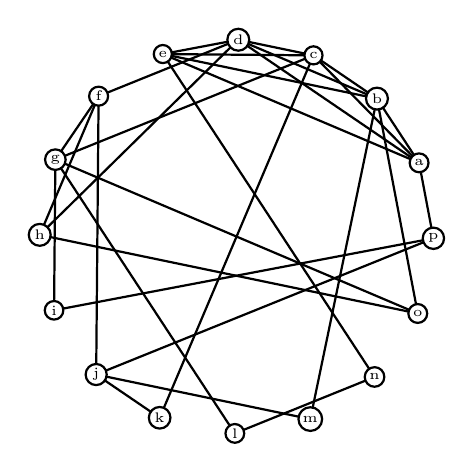
\begin{tikzpicture}[thick,scale=0.5]

	\coordinate (a1) at (22:5);
	\coordinate (a2) at (44.5:5);
	\coordinate (a3) at (67:5);
	\coordinate (a4) at (89.5:5);
	\coordinate (a5) at (112:5);
	\coordinate (a6) at (134.5:5);
	\coordinate (a7) at (157:5);
	\coordinate (a8) at (179.5:5);
	\coordinate (a9) at (202:5);
	\coordinate (a10) at (224.5:5);
	\coordinate (a11) at (247:5);
	\coordinate (a12) at (269.5:5);
	\coordinate (a13) at (292:5);
	\coordinate (a14) at (314.5:5);
	\coordinate (a15) at (337:5);
	\coordinate (a16) at (359.5:5);

	% the K_5
	\draw (a1) -- (a2);
	\draw (a1) -- (a3);
	\draw (a1) -- (a4);
	\draw (a1) -- (a5);
	\draw (a2) -- (a3);
	\draw (a2) -- (a4);
	\draw (a2) -- (a5);
	\draw (a3) -- (a4);
	\draw (a3) -- (a5);
	\draw (a4) -- (a5);

	% the connmatch
	\draw (a1) -- (a16);
	\draw (a2) -- (a13);
	\draw (a3) -- (a11);	
	\draw (a6) -- (a10); %new	
	\draw (a8) -- (a4);
	\draw (a5) -- (a14);
	
	% connect it up
	\draw (a6) -- (a4); 
	\draw (a6) -- (a8);
	\draw (a10) -- (a11);
	\draw (a10) -- (a13);
	\draw (a10) -- (a16);

	% the K_{1,3}
	\draw (a7) -- (a9);
	\draw (a7) -- (a15);
	\draw (a7) -- (a12);
	
	% connect THAT up
	\draw (a7) -- (a6);
	\draw (a7) -- (a3);
	\draw (a9) -- (a16);
	\draw (a15) -- (a2);
	\draw (a12) -- (a14);
	\draw (a15) -- (a8);
	% the nodes
	\draw (a1) node[lblvertex2] {a};
	\draw (a2) node[lblvertex2] {b};
	\draw (a3) node[lblvertex2] {c};
	\draw (a4) node[lblvertex2] {d};
	\draw (a5) node[lblvertex2] {e};
	\draw (a6) node[lblvertex2] {f};
	\draw (a7) node[lblvertex2] {g};
	\draw (a8) node[lblvertex2] {h};
	\draw (a9) node[lblvertex2] {i};
	\draw (a10) node[lblvertex2] {j};
	\draw (a11) node[lblvertex2] {k};
	\draw (a12) node[lblvertex2] {l};
	\draw (a13) node[lblvertex2] {m};
	\draw (a14) node[lblvertex2] {n};
	\draw (a15) node[lblvertex2] {o};
	\draw (a16) node[lblvertex2] {p};
	
\end{tikzpicture}
\end{center}
\caption{A graphical model of a social networking application}
\label{soc_net}
\end{figure}
When presented with any graph structure, one can immediately consider what systems the structure can model.  A graph model abstracts away the ``connectedness'' relationships of a complex system and views them out of context.  By determining the specific connectedness properties of the structure in question, one discovers the sort of systemic properties optimized by the presence of that structure. As a motivating hypothetical example, let us consider a social networking application with a mutual information sharing funtion between users (``friends'').  We derive a graphical model by assigning a vertex to represent each user, with an edge between vertices representing users that share information (figure \ref{soc_net}).

The presence of a clique in this model indicates a collection of users that pairwise share information.  The maximum clique problem has as its solution the largest such collection, illustrated in figure \ref{soc_net_clique}.
\begin{figure}[h]
\begin{center}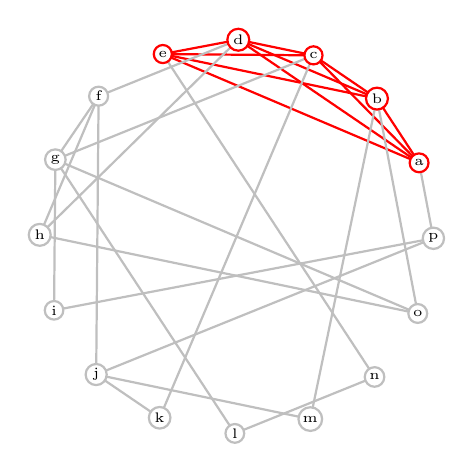
\begin{tikzpicture}[thick,scale=0.5]

	\coordinate (a1) at (22:5);
	\coordinate (a2) at (44.5:5);
	\coordinate (a3) at (67:5);
	\coordinate (a4) at (89.5:5);
	\coordinate (a5) at (112:5);
	\coordinate (a6) at (134.5:5);
	\coordinate (a7) at (157:5);
	\coordinate (a8) at (179.5:5);
	\coordinate (a9) at (202:5);
	\coordinate (a10) at (224.5:5);
	\coordinate (a11) at (247:5);
	\coordinate (a12) at (269.5:5);
	\coordinate (a13) at (292:5);
	\coordinate (a14) at (314.5:5);
	\coordinate (a15) at (337:5);
	\coordinate (a16) at (359.5:5);

	% the K_5
	\draw (a1)[red] -- (a2);
	\draw (a1)[red] -- (a3);
	\draw (a1)[red] -- (a4);
	\draw (a1)[red] -- (a5);
	\draw (a2)[red] -- (a3);
	\draw (a2)[red] -- (a4);
	\draw (a2)[red] -- (a5);
	\draw (a3)[red] -- (a4);
	\draw (a3)[red] -- (a5);
	\draw (a4)[red] -- (a5);

	% the connmatch
	\draw (a1)[black!25] -- (a16);
	\draw (a2)[black!25] -- (a13);
	\draw (a3)[black!25] -- (a11);	
	\draw (a6)[black!25] -- (a10); %new	
	\draw (a8)[black!25] -- (a4);
	\draw (a5)[black!25] -- (a14);
	
	% connect it up
	\draw (a6)[black!25] -- (a4); 
	\draw (a6)[black!25] -- (a8);
	\draw (a10)[black!25] -- (a11);
	\draw (a10)[black!25] -- (a13);
	\draw (a10)[black!25] -- (a16);

	% the K_{1,3}
	\draw (a7)[black!25] -- (a9);
	\draw (a7)[black!25] -- (a15);
	\draw (a7)[black!25] -- (a12);
	
	% connect THAT up
	\draw (a7)[black!25] -- (a6);
	\draw (a7)[black!25] -- (a3);
	\draw (a9)[black!25] -- (a16);
	\draw (a15)[black!25] -- (a2);
	\draw (a12)[black!25] -- (a14);
	\draw (a15)[black!25] -- (a8);

	% the nodes
	\draw (a1) node[lblvertex3, draw = red] {a};
	\draw (a2) node[lblvertex3, draw = red] {b};
	\draw (a3) node[lblvertex3, draw = red] {c};
	\draw (a4) node[lblvertex3, draw = red] {d};
	\draw (a5) node[lblvertex3, draw = red] {e};
	\draw (a6) node[lblvertex3] {f};
	\draw (a7) node[lblvertex3] {g};
	\draw (a8) node[lblvertex3] {h};
	\draw (a9) node[lblvertex3] {i};
	\draw (a10) node[lblvertex3] {j};
	\draw (a11) node[lblvertex3] {k};
	\draw (a12) node[lblvertex3] {l};
	\draw (a13) node[lblvertex3] {m};
	\draw (a14) node[lblvertex3] {n};
	\draw (a15) node[lblvertex3] {o};
	\draw (a16) node[lblvertex3] {p};

	
\end{tikzpicture}
\end{center}
\caption{Maximum clique, $\omega(G) = 5$}
\label{soc_net_clique}
\end{figure}  

Now suppose that our social networking application supports a ``group'' function wherein users may form groups with the property that group members expose information (reciprocally) with any users sharing information with any other member of the group.  If one can join a group only on the invite of a ``friend'', then the group formation process can be modeling by the sequential contraction of edges in the modeling graph.  Now information-sharing among groups can be modeled by minors found in the graph in the same way that the original graph models such sharing among individual users.

In particular, we can ask for the maximum number of groups that can be formed with the property that they pairwise share information.  In the model, this is tantamount to asking for the largest \textit{clique minor}.  In figure \ref{soc_net_minor}, each color indicated the edges to contract to form a collection of seven groups mutually sharing information.
\begin{figure}[h]
\begin{center}\input{party4}\end{center}
\caption{Maximum clique minor, $\eta(G) = 7$}
\label{soc_net_minor}
\end{figure} 

Connected matchings are a special case of clique minors.  In particular, every edge of a $k$-connected matching can contracted to form a copy of $K_k$.  In this application, asking for the maximum connected matching in out graphical model tells us the size of the largest collection of groups with \textit{exactly two members} that mutually share information. 
\begin{figure}[h]
\begin{center}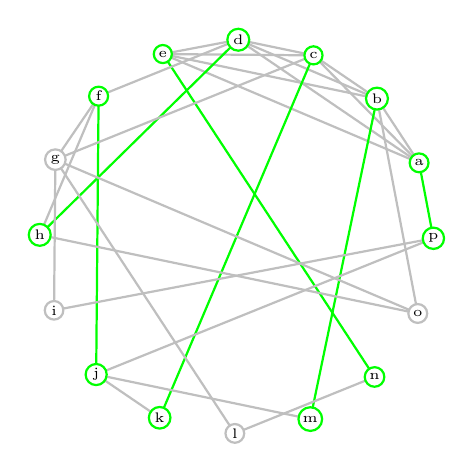
\begin{tikzpicture}[thick,scale=0.5]

	\coordinate (a1) at (22:5);
	\coordinate (a2) at (44.5:5);
	\coordinate (a3) at (67:5);
	\coordinate (a4) at (89.5:5);
	\coordinate (a5) at (112:5);
	\coordinate (a6) at (134.5:5);
	\coordinate (a7) at (157:5);
	\coordinate (a8) at (179.5:5);
	\coordinate (a9) at (202:5);
	\coordinate (a10) at (224.5:5);
	\coordinate (a11) at (247:5);
	\coordinate (a12) at (269.5:5);
	\coordinate (a13) at (292:5);
	\coordinate (a14) at (314.5:5);
	\coordinate (a15) at (337:5);
	\coordinate (a16) at (359.5:5);

	% the K_5
	\draw (a1)[black!25] -- (a2);
	\draw (a1)[black!25] -- (a3);
	\draw (a1)[black!25] -- (a4);
	\draw (a1)[black!25] -- (a5);
	\draw (a2)[black!25] -- (a3);
	\draw (a2)[black!25] -- (a4);
	\draw (a2)[black!25] -- (a5);
	\draw (a3)[black!25] -- (a4);
	\draw (a3)[black!25] -- (a5);
	\draw (a4)[black!25] -- (a5);

	% the connmatch
	\draw (a1)[green] -- (a16);
	\draw (a2)[green] -- (a13);
	\draw (a3)[green] -- (a11);	
	\draw (a6)[green] -- (a10); %new	
	\draw (a8)[green] -- (a4);
	\draw (a5)[green] -- (a14);
	
	% connect it up
	\draw (a6)[black!25] -- (a4); 
	\draw (a6)[black!25] -- (a8);
	\draw (a10)[black!25] -- (a11);
	\draw (a10)[black!25] -- (a13);
	\draw (a10)[black!25] -- (a16);

	% the K_{1,3}
	\draw (a7)[black!25] -- (a9);
	\draw (a7)[black!25] -- (a15);
	\draw (a7)[black!25] -- (a12);
	
	% connect THAT up
	\draw (a7)[black!25] -- (a6);
	\draw (a7)[black!25] -- (a3);
	\draw (a9)[black!25] -- (a16);
	\draw (a15)[black!25] -- (a2);
	\draw (a12)[black!25] -- (a14);
	\draw (a15)[black!25] -- (a8);

	% the nodes
	\draw (a1) node[lblvertex3, draw = green] {a};
	\draw (a2) node[lblvertex3, draw = green] {b};
	\draw (a3) node[lblvertex3, draw = green] {c};
	\draw (a4) node[lblvertex3, draw = green] {d};
	\draw (a5) node[lblvertex3, draw = green] {e};
	\draw (a6) node[lblvertex3, draw = green] {f};
	\draw (a7) node[lblvertex3] {g};
	\draw (a8) node[lblvertex3, draw = green] {h};
	\draw (a9) node[lblvertex3] {i};
	\draw (a10) node[lblvertex3, draw = green] {j};
	\draw (a11) node[lblvertex3, draw = green] {k};
	\draw (a12) node[lblvertex3] {l};
	\draw (a13) node[lblvertex3, draw = green] {m};
	\draw (a14) node[lblvertex3, draw = green] {n};
	\draw (a15) node[lblvertex3] {o};
	\draw (a16) node[lblvertex3, draw = green] {p};

	
\end{tikzpicture}
\end{center}
\caption{Maximum connected matching, $cm(G) = 6$}
\label{soc_net_conmatch}
\end{figure} 
It is worth noting that while $\omega(G)$ and $cm(G)$ are always less than or equal to $\eta(G)$ (as cliques and connected matchings are particular cases of clique minors), there is no such clear relationship between $\omega(G)$ and $cm(G)$.

\subsection{Computing connected matchings}
Now we take up the complexity of computing the largest connected matching in a graph.  We can define the computational problem as follows
{\linespread{1.2}\begin{framed}
  \noindent \textbf{Maximum Connected Matching (MCM)}
  \vskip 0.25 cm 
  \noindent Input: Graph $G$
  \newline Output: Maximum connected matching of $G$
 \end{framed}
We also may be interested in the largest connected portion of a given matching in $G$
 \begin{framed}
  \noindent \textbf{Maximum Connected Portion (MCP)}
  \vskip 0.25 cm 
  \noindent Input: A matching $M$ from a graph $G$
  \newline Output: Maximum connected portion of $M$
\end{framed}}
Both MCM and MCP are NP-hard in general.  Plummer et al. consider MCM in \cite{Spec_case}, and we will show a reduction of the maximum clique problem to MCP, verifying its hardness.  Cameron \cite{K_Cam} has shown that MCM remains hard even for bipartite graphs, while it is in $\mathbf{P}$ for chordal graphs.  Upon developing some machinery in the following section. we shall exhibit some results and further conjectures on classes of graphs with efficient solutions to these problems.



%\section{Proximity colorings}
	%\subsection{The proximity partition}
		%For any graph $G$ on $n$ vertices, there is a natural partition of the edges of a complete graph on $n$ vertices constructed by collecting each edge $uv$ into a distinct class $P_i = \{uv : d_G(u,v) = i\}$ .  We call this the \textit{proximity partition} $\mathcal{P}_G$ induced by $G$.  For an integer $k$, we can also consider the \textit{proximity $k$-partition} $\mathcal{P}^k_G$ induced by $G$, where for $1 < i < k$, $P_i = \{uv : d_G(u,v) = i\}$ and $P_k = \{uv : d_G(u,v) \geq k\}$. Occasionally, for small values of $k$, we may think of this partiton as an edge coloring of $K_n$ and refer to the \textit{proximity $k$-coloring} of $K_n$.  
\bprop{For any fixed $k$, determining whether a given partition of the edges $K_n$ is a proximity $k$-partition can be done in time polynomial in $n$.}

\begin{proof}
Suppose we have a partition $\mathcal{P}$ of the edges of $K_n$. If the $\mathcal{P}$ has more than $k$ classes, it clearly cannot be a proximity $k$-partition. Therefore there are at most $k!$ possible indexings of $\mathcal{P}$.  Checking whether a given indexing gives rise to a proximity $k$-partition can be accomplished in no more than $k$ matrix multiplications and comparisons.  
\end{proof}
In the case of a proximity $3$-coloring, we introduce a further shothand.  The RGB graph induced by a graph $G$ is the proximity $3$-coloring induced by $G$ with $P_1$ colored blue, $P_2$ colored green, and $P_3$ colored red.
\begin{prop}
Connected matchings in a graph $G$ correspond to green cliques in the RGB graph induced by $G$.  Copies of $2K_2$ correspond to red edges in the RGB graph induced by $G$.
\end{prop} 

The proximity partition induced by a graph $G$ can be thought of as the collection of \textit{distance-$k$ graphs} of $G$.  We may ask if there is a characterization of $\mathcal{H}_k$ where
\[\mathcal{H}_k = \{H :\: H \makebox{ is the distance-$k$ graph of some graph } G\}\]
In the case of $\mathcal{H}_2$, we can do so.  Let $A(G)$ denote the adjacency matrix of a graph $G$.  In \cite{sqrtofgraph} Mukhopdhyay characterizes graphs that have a \textit{square root}, which is to say graphs $H$ such that for some $G$, $A(H) = A(G)^2$.  This is equivalent to $H$ possesing an edge between any pair of vertices $u,v$ that satisfy $d_G(u,v) \leq 2$.  
\bthm{[Mudkhopdhyay] A connected graph $G$ with $n$ vertices $v_1, v_2, \ldots, v_n$ has a square root if and only if some set of $n$ complete subgraphs of $G$ whose union is $G$ can be labeled $C_1, C_2, \ldots, C_n$ so that, for all $i,j = 1, 2, \ldots, n$ the following conditions hold:
\begin{enumerate}
	\item $C_i$ contains $v_i$,
	\item $C_i$ contains $v_j$ if and only if $C_i$ contains $v_i$.
\end{enumerate}}
\noindent An alternate definition of $\mathcal{H}_2$ is 
\[\mathcal{H}_2 = \{H : \: A(H) = A(G)^2-A(G)\}\] and we have the following characterization in the spirit of Mukhopdhyay's theorem.  
\bthm{A graph $G$ with $n$ vertices $v_1, v_2, \ldots , v_n$ is the distance 2 graph of some graph $H$ if and only if some set of $n$ subgraphs of $G$ whose union is $G$ can be labeled $C_1, C_2, \ldots, C_n$ so that 
\begin{enumerate}
	\item $v_a \notin C_a$ 
	\item For every pair of vertices $v_i, v_j \in C_k$, exactly one of the following holds:
	\begin{enumerate}
		\item $v_iv_j \in E(C_k)$ 
		\item If $v_i \in V(C_j)$, then $v_j \in V(C_i)$
		\item $v_i \in C_j$ and $v_j \in C_i$
	\end{enumerate}
	\item If $C_i \cap C_j \neq \emptyset$, then $v_i, v_j \in V(C_k)$ for some $k$.
\end{enumerate}}
\begin{proof}
Suppose we have a graph $G$ on vertices $v_1, v_2, \ldots, v_n$ and subgraphs $C_1, C_2, \ldots, C_n$ that satisfy the above hypotheses.  We construct a graph $H$ on the same vertex set by adding edges in two steps for each $C_i$.
\begin{description}
	\item[Step 1.] Add the complement of $C_i$.
	\item[Step 2.] Add all edges from $v_i$ to $C_i$.
\end{description}
	We claim that $G$ is now the distance 2 graph of $H$.  Suppose that $d_H(v_i, v_j) = 2$.  We want to show that $v_iv_j \in E(G)$.  Since $d_H(v_i,v_j) \leq 2$, there is some vertex $v_k$ so that $v_iv_k, v_jv_k \in E(H)$.  If both edges were added in step 2, then one of the following occurs
\begin{description}
	\item[Case 1.] $v_i, v_j \in C_k$
	\item[Case 2.] $v_k \in C_i$, $v_k \in C_j$
	\item[Case 3.] $v_k \in C_i, C_j$
\end{description}    
In case 1, distance 2 implies $v_iv_j \notin E(H)$. In particular, this edge was not added in step 2, so $v_i \notin C_j$ and $v_j \notin C_i$.  Condition 2 then implies that if $v_i, v_j \in C_k$ for some $C_k$, then $v_iv_j \in E(G)$.  In case 2, $V(C_i)$ and $V(C_j)$ intersect, implying (by condition 3) again that there is a $V(C_l)$ containing both $v_i$ and $v_j$.  In case 3, condition 4 requires that $v_i, v_j \in C_k$.  In any event, $v_iv_j \in E(G)$.

Now we may assume WLOG that $v_iv_k$ was added to $H$ in step 1.  Suppose $v_jv_k$ was added in step 2. Then either $v_k \in C_j$, implying $C_i \cap C_j \neq \emptyset$, or $v_j \in C_k$ implying $v_i, v_j \in C_k$.  The only remaining possibility is that both $v_iv_k$ and $v_jv_k$ were added in step 1.  Following from two applications of condition 2(b), both $v_i$ and $v_j$ are then in $V(C_k)$.  Sufficiency complete.

For the proof of necessity, we take a graph $H$ and show that its distance two graph $D_2(H)$ has a collection of subgraphs with the necessary properties.  For each vertex $v_i$, let $V(C_i) = N(v_i)$.  That condition 1 holds is immediate.  The vertices of any given $C_i$ are at most distance two apart.  Whenever there is a nonedge in a particular $C_i$ and 2(a) fails, the vertices must be adjacent in $H$, and condition 2(b) holds.  The symmetric property of the neighbor relation shows that conditions 3 and 4 hold as well.  Finally, all distance 2 edges occur between vertices with a common neighbor, so $\bigcup C_i = G$. 
\end{proof}



%\section{Computational results}
	%\subsection{Hardness of MCP}
Considering the RGB graph induced by some underlying graph, we can easily apply known complexity results regarding the maximum clique problem to explore the complexity of MCM and MCP.  First, we will determine the hardness of MCP.
\begin{theorem}
	MCP is NP-hard.
\end{theorem}
This can be easily seen by demonstrating that any maximum clique problem can be formulated as an MCP problem
\begin{lem}
	Any graph $G$ has a realization as the green edges in the RGB graph induced by a matching in some graph $H$.
\end{lem}
\begin{proof}
	Let $G$ be an arbitrary graph.  For every vertex of $G$, add one copy of $K_2$ to $H$.  If and only if vertices $u,v$ are adjacent in $G$, add an edge between some endpoints of the corresponding copies of $K_2$ in $H$.
\end{proof}
Note that a similiar proof of the NP-hardness of MCM is impossible, as not every graph can be realized as the entire green graph of an RGB graph.
\subsection{Efficent classes}
By reducing connected matching problems to clique problems we can describe some classes of graphs that have efficient conneected matching algorithms.  Most essentially we have the following.
\begin{theorem}
	Let $\mathcal{S}$ be a graph property for which MAX CLIQUE has an efficient solution.  Then if $\mathcal{S'}$ is the class of graphs that induce RGB graphs such that the green edges induce a memeber of $\mathcal{S}$, then MCM is efficient for $\mathcal{S'}$. 
\end{theorem} 
Understanding this relationship of graph properties is ongoing work.

In the case of MCP, we can describe the following polytime-recognizable class of graphs wherein MCM $\in$ \textbf{P}.
\begin{prop}
	If the RGB graph induced by a matching $M$ in a graph $M$ has a red graph that is bipartite, then MCP has a polytime soluton for $G$ and $M$.
\end{prop}


%\section{The extremal connected matching conjecture}
	%\subsection{An easy lemma}
		\begin{prop}
	If SSH holds for a \kfree graph $G$ with $n$ vertices, then $\nu_c(G) \geq \frac{1}{4}n$. 
\end{prop}
\begin{proof}
	Let $\mathcal{M}$ be the collection of branch sets of a $n/2$ SSH-minor of $G$.  Let $\mathcal{M}_1 = \{M\in \mathcal{M}: |M| = 1\}$ and $\mathcal{M}_2 = \{M\in \mathcal{M}: |M| = 2\}$. Then 
\[\nu_c(G) \geq \frac{1}{2}|\mathcal{M}_1| + |\mathcal{M}_2| \geq \frac{1}{2}(|\mathcal{M}_1| + |\mathcal{M}_2|) = \frac{1}{4}n\]
\end{proof}
In Lemma 2.1 of \cite{blas}, Blasiak shows that \kfree graph with connectivity less than $n/2$ satisfies SSH.  We can show the following for higher connectivity.
\begin{lem}
	If $G$ is a \kfree graph on $n$ vertices with $\kappa(G) \geq n/2$, then $\nu_c(G) \geq n-\kappa(G)$.  (Further, if $n/4 < \kappa(G) < n/2$, then $\nu_c(G) \geq \kappa(G)$ and if $\kappa(G) < n/4$ then $\nu_c(G) \geq \frac{1}{4}(n-\kappa(G)$ maybe more) 
\end{lem}
\begin{proof}
	The proof begins similarly to \cite{blas}. Let $S$ be a minimum cut set of $G$.  Then let $L$, $R$ be a partition of $V(G) - S$ so that $L$ and $R$ do not touch.  Since $G$ is \kfree, $L$ and $R$ are cliques, and every vertex of $S$ is complete to $L$ or complete to $R$.  Let $S_L$ be the set of vertices complete to $L$ and $S_R$ the set of vertices complete to $R$.    We claim that between any $A \subseteq S_L$ with $|A| \leq |R|$ and $R$ ($S_R$ and $L$ resp.) there is a matching that saturates $A$.  Suppose there is no $(A, R)$ matching saturating $A$.  Hall's condition then implies that there is $T\subseteq A$ such that $|N(T)\cap R| < |T|$. But then $(S-T)\cup (N(T)\cap R)$ is a cut set separating $L\cup T$ and $R-N(T)$. This set is smaller than $S$, yielding a contradiction.   

Let $M$ be the largest possible matching obtained with $(S_L,R)$ edges and $(S_R,L)$ edges.  This matching is connected, and $|M| = \min\{|S_L|, |R|\} + \min\{|S_R|, |L|\}$.  If both $|R| \leq S_L$ and $|L| \leq S_R$, then we are done.  If, WLOG,  $|R| > S_L$, then let $U_R$ denote the set of vertices of $R$ unmatched by $M$.  Since $|S|\geq n/2$, there are at least $|U_R|$ unmatched vertices of $S_R$ (denoted $U_{S_R}$).  Augment $M$ with any $(U_R , U_{S_R})$ matching saturating $U_R$ to yield $M'$.  These new edges are mutually connected, and connected to any $(S_R,L)$ or $(S_L, R)$ edges via $R$.  Hence, $M'$ is a $(S,S^c)$ connected matching saturating $S^c = R\cup L$, and $|R\cup L| = n-\kappa(G)$. 
\end{proof}



F\"{u}redi et. al note that the stronger version of conjecture \ref{c_conj} is sharp by exhibiting by the $\overline{K_3}$-free graph formed by a disjoint pair of cliques.  In general, if we consider only $\overline{K_3}$-free graphs with sufficiently large cliques it is easy to show that conjecture \ref{c_conj} holds.
\begin{lem}Let $0<c<1/4$.  If $G$ ($\alpha(G) \leq 2$) has $\omega(G) \geq cn$, then $G$ has a $(cn)$-connected matching.
\label{spider}
\end{lem}
\begin{proof}
	Let $S$ be a set of $cn$ vertices inducung a clique.  For any subset of $S'\subseteq S$, the intersection $\displaystyle I = \bigcap_{s\in S'} \{v \in V(G): sv \notin E(G)\}$ induces a clique.  If for any $S'\subseteq S$, $|I| > n/2$, then there is a $cn$-connected matching in the clique induced by $I$.  Otherwise, $|N(S')| \geq |S'|$ for all $S'\subseteq S$, and there is an $S-(V(G)-S)$ matching saturating $S$.  This matching must be connected, since $S$ induces a clique. (This lemma appears implicitly in \cite{FGS})
\end{proof}
This lemma immediately yields several properties that a minimal counterexample to conjecture \ref{c_conj} must possess.
\begin{prop}
 If $G_{c'}$ is a vertex minimal counter example to conjecture \ref{c_conj} with $c = c'$, then the following hold 
\begin{enumerate}
	\item $\omega(G_{c'}) < c'n$
	\item $G_{c'}$ and $\overline{G_{c'}}$ have diameter 2
	\item $G_{c'}$ has no edge dominating $n-c'$ vertices
	\item $\delta(G_{c'}) \geq (1-c')n$.
	\item $G_{c'}$ is $(1-2c')n$-connected.
\end{enumerate}
\end{prop}

	%\subsection{The Ramsey bound}
		%+In \cite{MR1369063}, Kim famously proved that the magnitude of the Ramsey number $R(3,k)$ is $\Theta(k^2/\log k)$.  This means that for any fixed $c$ there are graphs that do not meet the hypotheses of lemma \ref{spider}.  The so-called \textit{Ramsey graphs}, in this case $\overline{K_3}$-free graphs with clique number within a constant multiple of the Ramsey bound, do not have large enough cliques.  However, for sufficiently large Ramsey graphs, we can show that conjecture \ref{c_conj} holds, and that the value of $c$ is arbitrarily close to $1/4$. 

\begin{theorem}
Let $c < 1/4$ be a constant.  For any constant $b$ and sufficently large $n$, every $\overline{K_3}$-free graph $G$ on $n$ vertices with $\omega(G) < b\sqrt{n\log n}$ has a $cn$-connected matching.
\label{sm_cli}
\end{theorem}

We will employ the following lemma about triangle free graphs with small independence number.

\begin{lem}
For every pair of positive constants $\epsilon, d$ there is $n_{\epsilon, d}$ such that every triangle-free graph $G$ with $n > n_{\epsilon, d}$ vertices and $\alpha(G) < d\sqrt{n\log n}$ has fewer than $\epsilon n^3$ copies of $C_4$.
\end{lem}
\begin{proof}
Fix $\epsilon, d> 0$ and let $G$ be a triangle free graph on $n$ vertices with $\alpha(G) < d\sqrt{n\log n}$.  Let $X_{C_4}$ be the number of $C_4$ in $G$.  Then
\[X_{C_4} = \frac{1}{2}\sum_{\{u,v\}\notin E(G)} {|N(u) \cap N(v)| \choose 2}\]
Set $\epsilon_1 = \sqrt{8\epsilon}$.

\noindent\textit{Claim. For sufficiently large $n$, fewer than $n^2(\log n)^{-2}$ pairs of vertices $u,v$ have neighborhood intersection larger than $\epsilon_1\sqrt{n}$.}

Suppose the contrary is true, and there are more than $n^2(\log n)^{-2}$ pairs $u,v$ so that $|N(u)\cap N(v)| \geq \epsilon_1\sqrt{n}$. When we count the total number of vertices in these intersections, the count is at least $\epsilon_1n^{5/2}(\log n)^{-2}$, meaning some vertex is counted $\epsilon_1n^{3/2}(\log n)^{-2}$ times.  However, $\Delta(G) \leq \alpha(G) < d\sqrt{n\log n}$, so each vertex is in at most \[{d\sqrt{n\log n}\choose 2 } < \frac{d^2}{2}n\log n\] neighborhood intersections.  Thus, for sufficiently large $n$,  the claim holds.

Now we can bound $X_{C_4}$.
\begin{eqnarray}X_{C_4} <& \frac{1}{2}\left[\frac{n^2}{(\log n)^2}{d\sqrt{n\log n}\choose 2}+ \left(|E(\overline{G})|- \frac{n^2}{(\log n)^2}\right){\epsilon_1\sqrt{n}\choose 2}\right]\\
\sim& \frac{\epsilon_1^2}{8}n^3 = \epsilon n^3
\end{eqnarray}
Thus for sufficiently large $n$, $X_{C_4} < \epsilon n^3$.
\end{proof}
\vskip 1 cm
 
Now we can prove theorem \ref{sm_cli}.

\begin{proof}[Proof (of Theorem 1)]
Fix constants $d$ and $c < 1/4$, and let $G$ be a $\overline{K_3}$-free graph with $n$ vertices, $m$ edges, and $\omega(G) < b\sqrt{n\log n}$.  Consider the $RGB$ graph $\mathcal{G}$ sinduced by $G$ (recalling that green $k$-cliques correspond to $k$-connected matchings in $G$ and red edges correspond to induced $\overline{C_4}$s in $G$).  If $R, G,$ and $B$ denote the number of red, green and blue edges respectively, we would like to show that \[G = {m\choose 2} - R - B \geq {m\choose 2} - cn{m/cn\choose 2}\] equivalently
\begin{equation}
	R + B \leq cn{m/cn\choose 2}\label{goal}
\end{equation}
guaranteeing by T\'{u}ran's theorem (see, \textit{e.g.}, \cite{dwest}) a green clique on $cn$ vertices in $\mathcal{G}$, and a $cn$-connected matching in $G$.

We obtain a crude upper bound on $B$ by taking the number of edges in the line graph of $K_n$.
\begin{equation}
	B < \frac{n^3}{2} - \frac{3n^2}{2} + n
\end{equation}
We can also asymptotically bound $R$ using Lemma 1.  For any $\epsilon > 0$ and sufficiently large $n$, \[B + R < \frac{n^3}{2} + \epsilon n^3\]
We compare this with the right hand side of (\ref{goal})
\begin{eqnarray}
	cn{m/cn\choose 2} =&\displaystyle \frac{cn}{2}\left(\frac{m^2}{c^2n^2} - \frac{m}{cn}\right)\\
	=& \displaystyle \frac{1}{2c}m^2n^{-1} - \frac{m}{2}\\
	\sim&   \displaystyle \frac{n^3}{8c}
\end{eqnarray}
Since $c < 1/4$, and we can take $\epsilon < \frac{1-4c}{8c}$, for sufficiently large $n$ (\ref{goal}) holds and $G$ has a $cn$-connected matching.
\end{proof}
The \textit{triangle free process} is a method of stochastically constructing maximal triangle free graphs.  Let $G_0$ be the empty graph on $n$ vertices and let $O_i$ be the set of edges of $K_n- G_i$ that will not create a triangle when added to $G_i$.  Then for each $G_i$, construct $G_{i+1}$ by adding an edge chosen uniformly at random from $O_i$ until some step $k$ at which $O_k$ is empty.  The complementary version of this process is a natural source of $\overline{K_3}$-free graphs.  It is worth noting, therefore, that Bohman has shown in CITE that the triangle free process (asymptotically almost surely) produces graphs which satisfy the hypotheses of Theorem \ref{sm_cli}.   



%\input{references}

\end{document}
